\documentclass[a4paper]{article}
\usepackage{graphicx}
\usepackage{amsmath, amsfonts, geometry, float, listings, enumerate, multicol}
\usepackage{multicol, float, color, colortbl}
\usepackage{tikz, titlesec, parskip}

\titlespacing{\section}{0pt}{10pt}{0pt}
\titlespacing{\subsection}{0pt}{10pt}{0pt}
\titlespacing{\subsubsection}{0pt}{10pt}{0pt}

\usetikzlibrary{calc,patterns,through}
\newcommand{\arcangle}{%
	\mathord{<\mspace{-9mu}\mathrel{)}\mspace{2mu}}%
}

\renewcommand{\baselinestretch}{1.2}
 \geometry{
 a4paper,
 total={170mm,257mm},
 left=20mm,
 top=20mm,
 }
\usepackage{fancyhdr}
\pagestyle{fancy}
\fancyhf{}
\rhead{\textbf{مقدمه‌ای بر یادگیری ماشین}}
\lhead{\textbf{تمرین سری اول}}
\cfoot{(\space \space \space \space \textbf{\thepage}  \space \space \space)}
\renewcommand{\headrulewidth}{1pt}
\renewcommand{\footrulewidth}{1pt}
 
\usepackage{xepersian}
%\setlatintextfont{Times New Roman}
\settextfont{XB Niloofar}
\setdigitfont{XB Niloofar}
\DefaultMathsDigits
\usepackage{amsmath}
\usepackage{pgfplots}
\tikzset{declare function={unitstep(\x)=notless(\x,0);}}
\tikzset{declare function={delta(\x)=equal(\x,0);}}

\begin{document}
\begin{minipage}{0.6\textwidth}

\begin{center}
	\begin{bf}
	باسمه تعالی\\
	\vspace{0.25cm}
	دانشگاه صنعتی شریف\\
	\vspace{0.25cm}
	دانشکده مهندسی برق\\
	\vspace{0.5cm}

\large
مقدمه‌ای بر یادگیری ماشین -دکتر جمال‌الدین گلستانی\\
\vspace{0.3cm}
\normalsize
بهراد منیری - ۹۵۱۰۹۵۶۴\\
\Large
\vspace{0.3cm}
گزارش بخش کامپیوتری تمرین سری اول\\
\vspace{0.4cm}
\end{bf}
\end{center}
\normalsize
\end{minipage} \hfill
\begin{minipage}{0.35\textwidth}

\begin{flushleft}
\includegraphics[width=0.6\textwidth]{Shariflogo.png}\\ \large
\end{flushleft}

\end{minipage}
\section{تمرین اول}
شکل زیر، نمودار‌های 
\lr{Scatter Plot}
داده‌های این تمرین، برای هر ویژگی هستند. داده‌های تست ، با رنگ قرمز و داده‌های آموزشی، با رنگ آبی مشخص شده‌اند.
\begin{figure}[h]
	\centering
	\includegraphics[width=\textwidth, height=0.4\textheight]{figs-q1.eps}
\end{figure}
\subsection{بخش الف}
ویژگی $X$ برای رگرسیون مناسب است اگر $X$ و $y$ مستقل نباشند. برای سنجش استقلال متغیر‌های تصادفی، می‌توان از آزمون فرضیه‌ی 
\lr{Hilbert-Schmidt}
استفاده کرد. با توجه به نمودار‌های، به صورت شهودی، به نظر می‌رسد که ویژگی شماره‌ی هشت بیشترین وابستگی را به $y$ داشته باشد و در نتیجه مناسب‌ترین انتخاب برای عمل رگرسیون است. بدترین ویژگی نیز ویژگی شماره‌ی ۳ است که به نظر مقدار‌ آن کاملاً مستقل از $y$ است.

\subsection{بخش ب}
 در متلب، به کمک نتایجی که در کلاس برای کمینه‌کردن 
 \lr{MSE}
 به دست آمد، رگرسیون خطی انجام می‌دهیم و خطای این رگرسیون را، یک بار بر روی خود داده‌های آموزشی، و یک بار بر روی داده‌های کنار‌گذاشته‌شده در یادگیری محاسبه می‌کنیم. در این‌جا نیز از 
  \lr{Squared Error}
  برای خطا استفاده می‌کنیم. مطابق انتظار، خطا بر روی داده‌های آموزشی، کم از از خطا بر روی داده‌های تست به دست آمد.


مقدار تلف، برای داده‌های تست، 
\lr{True Risk}،
برابر
$5.598\times10^3$
و برای داده‌های آموزشی،
\lr{Empirical Risk}،
$4.726\times10^3$
به دست آمد. بردار ضرایب نیز برابر
$$
\omega =
10^3 \times
[-0.04169,
-0.04186,
0.00117,
-0.00001,
0.00010,
-0.00004,
0.00006,
0.03896,
-3.48358]$$


\section{تمرین دوم}
داده‌‌ها را در محیط دوبعدی رسم می‌کنیم و آنها را با چند‌جمله‌ای هایی از درجات مختلف رگرس می‌کنیم. نقاط آبی، داده‌های و نقاط قرمز، پیش‌بینی ما برای داده‌های آموزشی است.
\begin{figure}[h]
	\centering
	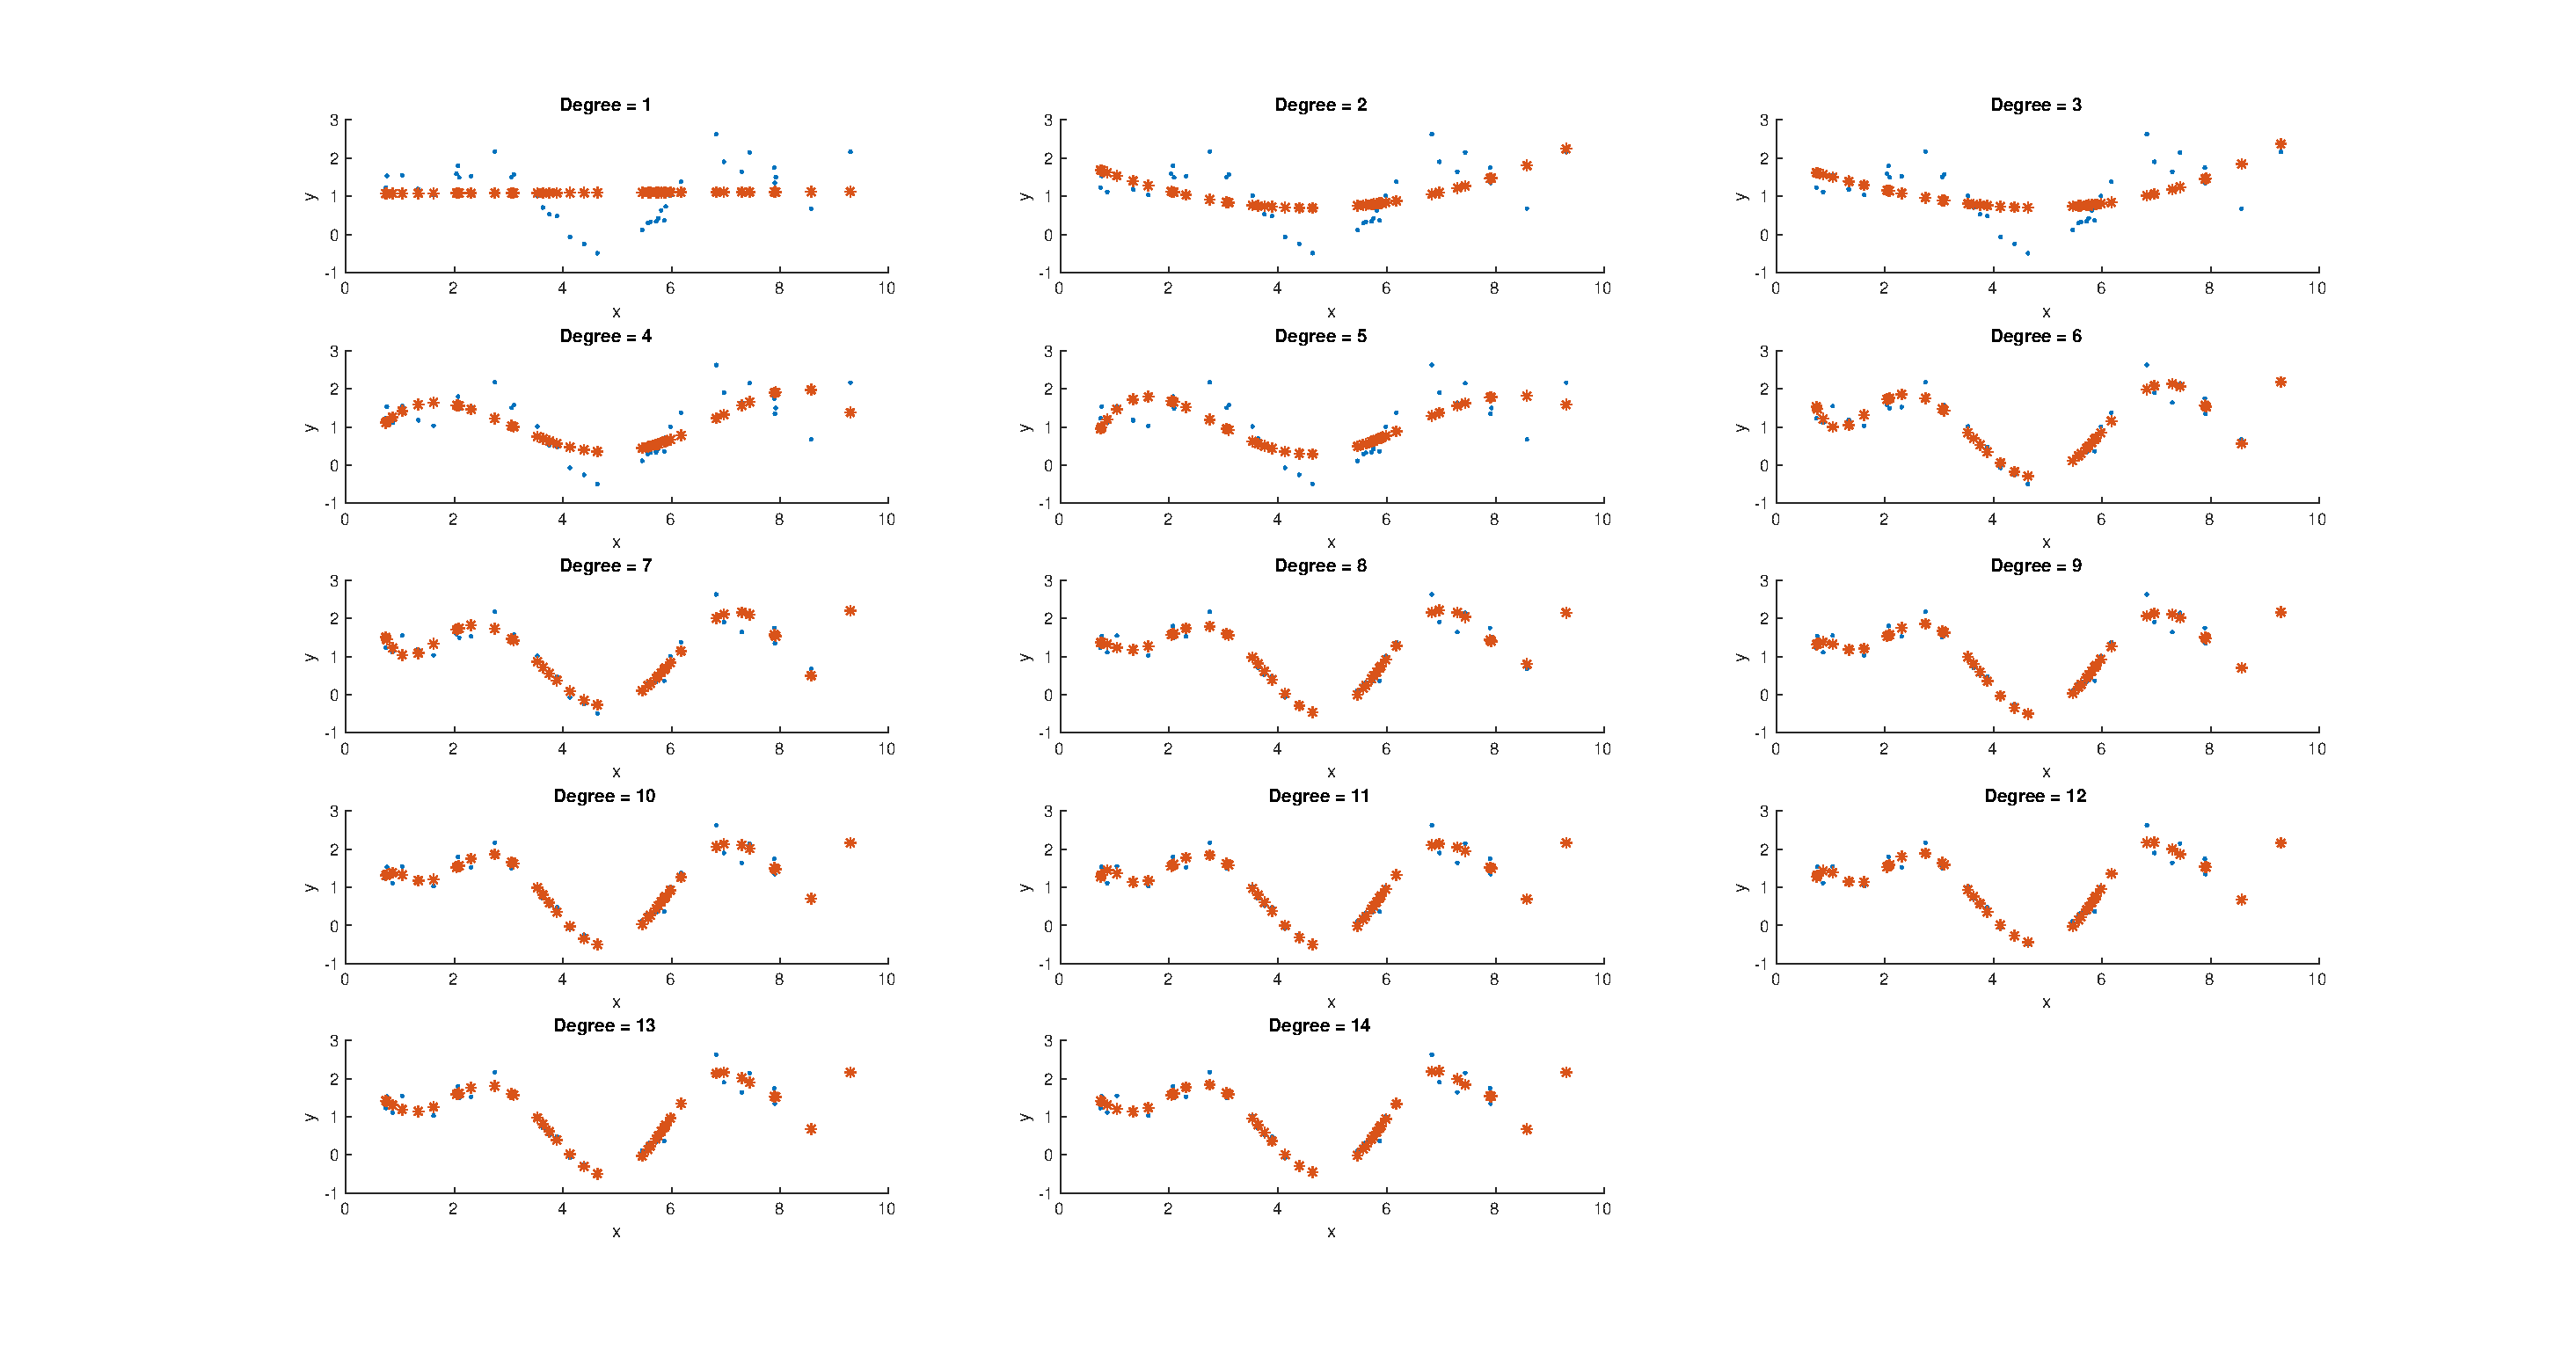
\includegraphics[width=\textwidth, height=0.4\textheight]{15.eps}
\end{figure}

 نمودار 
\lr{Empirical Risk}
و 
\lr{True Risk}
بر حسب درجات مختلف چندجمله‌ای، به صورت زیر است.
\begin{figure}[h]
	\centering
	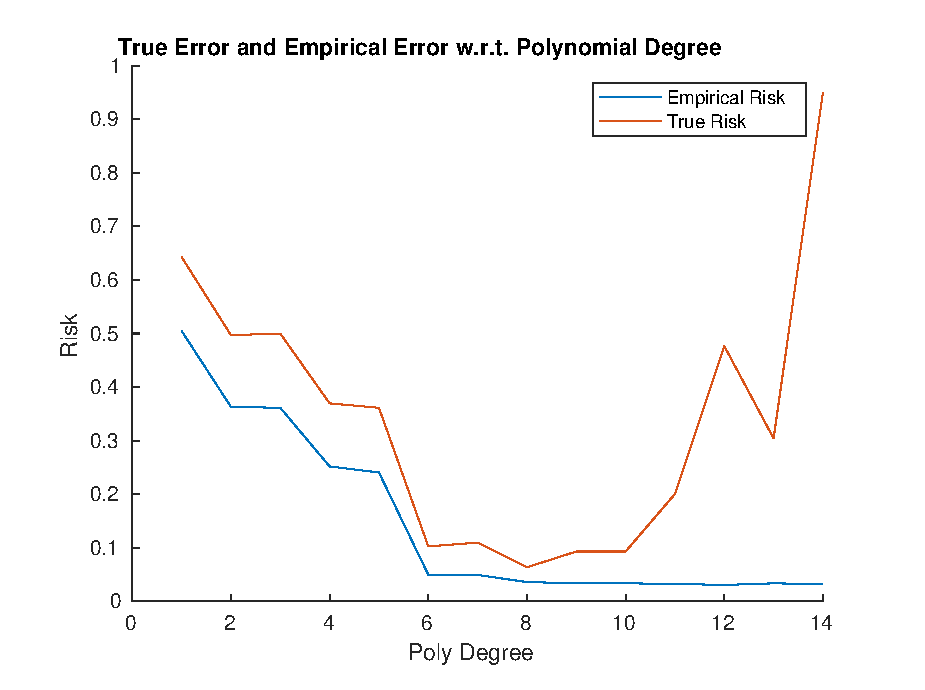
\includegraphics[scale = 0.8]{curves.eps}
\end{figure}

خطای واقعی به ازای چندجمله‌ای درجه‌ی هشت کیمنه می‌شود. 

همان‌طور که در درس دیدیم، با زیاد کردن درجه، کلاس فرضیه‌های خود را بزرگتر می کنیم و در نتیجه خطا بر روی داده‌های آموشی کمتر می‌شود یا ثابت می‌ماند. این اتفاق به وضوح در نمودار دیده می‌شود. 
خطای واقعی نیز با غنی کردن مجموعه‌ی فرضیه‌های کاهش می‌یابد ولی بزرگ‌کردن بیش از حد آن باعث می‌شود تا دچار
\lr{Overfitting}
شویم.


\end{document}